\chapter{Power Up Unlocked!}
In this chapter we'll expand on some things we explored in the previous part, namely recursion and incidence 
matrices. Recursion is the mathematical version of the principle "We can't do the same thing again and 
again and expect different results". \par
Incidence matrices is another way to perform double counting to solve much more complicated questions.\par
This chapter is the start of our PnC journey away from short answer contests towards a more involved, 
more rigorous PnC.
\section{Recursion}
\begin{example}
[Motivating Example]
A tower of $n$ circular discs of different sizes is stacked on one of the 3 given pegs in 
decreasing size from the bottom. The task is to transfer the entire tower to another peg by 
sequence of moves under the
following conditions:\par 
(i) each moves carries exactly one disc, and\par 
(ii) no disc can be placed on top of a smaller one.\par
It is said that there is temple in Kashi where in its basement are priests playing this game 
with $64$ discs. They started playing at the dawn of time and when they finish the universe will 
die. Considering it takes them $1$ sec to move a disc, how long do we have?
\end{example}
\begin{proof}
    [Solution]
    $64$ discs seem quite a lot to work with. Let's look at a Small case.
    If they had $1$ disc, it would take them $1$ move.\par
    If they had $2$ discs, it would take $3$ moves.\par
    If they had $3$ discs, it would take $7$ moves, as illustrated below:\par
    \begin{figure}[H]
        \centering
        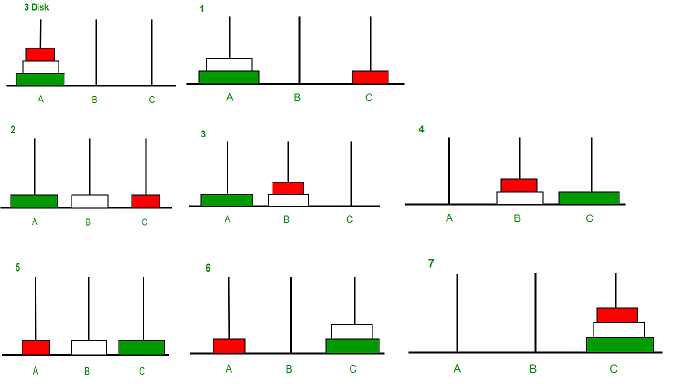
\includegraphics[width=0.5\linewidth]{Tower of hanoi at n=3.png}
    \end{figure}
    We can see a pattern here. For some $n$, let $M_n$ be the moves required. 
    Then $M_{n+1}=2M_{n}+1$ Let's prove it now.\par
    Lets consider it took some $M_n$ moves to move $n$ discs.\par
    So to move $n+1$ discs we first move the top $n$ discs to the second pole in 
    $M_n$ moves. We then move the largest disc to third pole in $1$ move. We then finally move the 
    $n$ discs to the third pole in $M_n$ moves.\par
    This means it takes a total of $2M_n+1$ moves to move $n+1$ discs. 
    This is called the recusive formula as values of every term depends on the previous terms.\par
    We can try to find the explicit formula of $M_n$ for any $n$ by observing that $M_1=1=2^1-1$\par
    Which we can put into the recursive formula to get the form $M_n=2^n-1$\par
    For $n=64$, we will get such a big number that even in seconds that is $42$ times the 
    scientific life of universe.
\end{proof}
While the temple story is great, its fictional. It was created by a friend of Edward Lucas, 
the mathematician behind this game. There are some more versions of this problem which will 
make an appearance in the exercises.
\section{Fibonacci Sequence}
Any discussion on recurrence is incomplete without a discussion of the famous Fibonacci Sequence.\par
$1,1,2,3,5,8,13 \dots$ \par is a sequence at the heart of math and nature. 
We can see it in plants, animals to in the great pyramids to temples of Greece.\par
What makes this sequence so special?\par
It is the simplest form of recursion defined by $F_n=F_{n-1}+F_{n-2}$.\par
But it gets better!\par
\begin{example}
(IMO/3 1981) Determine all $(m,n)$ where $\displaystyle m$ 
and $\displaystyle n$ are integers satisfying 
$\displaystyle ( n^2 - mn - m^2 )^2 = 1$.
\end{example}
\begin{proof}
    [Solution]
We need to first see that $(n^2-mn-m^2)^2=1 \implies n^2-mn-m^2=\pm1$\par 
We can see that  $(m,n)=(1,1)$ is a solution, so is $(m,n)=(1,2)$ and so is $(m,n)=(2,3)$.\par
FIBONACCI!\par
We'll just need to prove this now.\par
Claim: If and only if $(m,n)$ is a solution than so is $(n,m+n)$.\par
Let $(n^2-mn-m^2)^2=1$ then:
\begin{align*}
((m+n)^2-(m+n)n-n^2)^2\\
=(m^2+\cancel{2}mn+\cancel{n^2}-\cancel{mn}-\cancel{n^2}-n^2)^2\\
=(m^2+mn-n^2)^2\\
= (-(m^2+mn-n^2)^2\\
= (n^2-mn+m^2)^2\\
=1
\end{align*}
This proves the if. To prove the only if, we'll argue as follows.\par
Let's assume, to the contrary, that there is some $(n,m+n)$ which is a solution but $(m,n)$ is not a solution.\par
This means $(m^2+mn-n^2)^2=1$  and $(n^2-mn+m^2)^2 = (-(m^2+mn-n^2))^2 = (m^2+mn-n^2)^2 \neq 1$\par
This is absurd!\par
Hence, contradiction. Thus, our initial claim must be false and there exists no such $(n,m+n)$\par
With this we have proven our claim.
\end{proof}
We'll see Fibonacci occur in other places as well.\par
For our further purposes, we ask ourselves how do we find the 
$500th$ Fibonacci number without needing to find the other $499$? 
Or basically what is the closed form of Fibonacci numbers?
\section{Solving Liner Recursion}
A linear recursion(where we the power/exponent of previous terms is $1$) can be solved 
to get it as a difference of some geometric progressions. However, determining 
them is a bit more invloved.\par
\begin{definition}[Characteristic polynomial]
Let $x_1,x_2,x_3 \dots$ be a series 
following the recurrence 
\[x_k=c_{k-1}x_{k-1}+c_{k-2}x_{k-2}+c_{k-3}x_{k-3} \dots\]
where $c$ refers to the coefficients of the terms in the recurrence relation. Then, 
the characteristic polynomial of the recurrence is:        
\[x^k=c_{k-1}x^{k-1}+c_{k-2}x^{k-2}+c_{k-3}x^{k-3} \dots\]
When we cancel the common powers, we will be left with the simplified characteristic polynomial.
\end{definition}
For example, for the Fibonacci numbers, we have:
\begin{align*}
F_n=F_{n-1}+F_{n-2}\\
\implies x^n=x^{n-1}+x^{n-2} \\
\implies x^2=x^1+1
\end{align*}
This is the characteristic polynomial. What is so special about this?
\begin{theorem}[Expanded form]
If the roots of the characteristic polynomial P are $r_1, r_2, r_3 \dots$ then there exist $a_1, a_2, a_3 \dots$:
\[x_n=a_1r_1^n+a_2r_2^n \dots\]
Here, if given the initial values of $x_n$ we can find $a_1, a_2 \dots$
\end{theorem}
This theorem is proven by (strong) induction. You can give it a try but 
I am not discussing it as it is quite long and tedious and unnecessary. 
What I will discuss is how to use this to find the $n^{th}$ Fibonacci number.
\section{Binet's Formula}
We can replace all $F_k$ with $x_k$. Thus,
\[x_k = x_{k-1} + x_{k-2},\]
implying
\[
x^2 - x - 1 = 0.
\]

The solutions to this equation are
\[
x_{1,2} = \frac{1 \pm \sqrt{1 + 4 \cdot (-1) \cdot (-1)}}{2} = \frac{-1 \pm \sqrt{5}}{2}.
\]

Thus, the formula must be of the form
\[
F_n = a_1 \left(\frac{-1 + \sqrt{5}}{2}\right)^n + a_2 \left(\frac{-1 - \sqrt{5}}{2}\right)^n,
\]
for constants $a_1$ and $a_2$. To find these two constants, we simply plug in $n = 0$ and $n = 1$ and get the desired result.
\par
If you solve for $a_1$ and $a_2$, you'll reach the result: $a_1=a_2=\frac{1}{\sqrt5}$.
\par
Putting that in the expression we get:
\[
F_n = \frac{\left(\frac{-1 + \sqrt{5}}{2}\right)^n + \left(\frac{-1 - \sqrt{5}}{2}\right)^n}{\sqrt5},
\]
This is known as the Binet Formula for the $n^{th}$ Fibonacci number. 
While you'll not get to use this formula a lot, but isn't amazing that despite being 
filled with so many $\sqrt5$ which are irrational, we will always get an positive integer. \par
Think about it...
\section{But Wait, what if the roots repeat?}
Nice question, let's look at an example from INMO 1996.
\begin{example}
The sequence $\{a_n\}_{n\in \mathbb{N}}$ is defined by $a_1=1, a_2=2,$ and $a_{n+2}=2a_{n+1}-a_n+2$ for $n \geq 1$.
Prove that for any $m$, $a_m a_{m+1}$ is also a term of the sequence.
\end{example}
\begin{proof}
    This example illustrates two concepts. First is what to do if we have a constant in the recurrence.\par
  We are given  $a_{n+2}=2a_{n+1}-a_n+2$, which means $a_{n+3}=2a_{n+2}-a_{n+1}+2$. Let's subtract them.\par
  $a_{n+3}-a_{n+2}=2a_{n+2}-3a_{n+1}+a_n$\par
  $\iff a_{n+3}=3a_{n+2}-3a_{n+1}+a_n$\par
  We can solve this recurrence. Let's make a characteristic pronominal,\par
  $x^3=3x^2-3x+1$\par
  $\iff x^3-3x^2+3x-1=0$\par
  $\iff (x-1)^3=0$\par
  Thus, we have all three roots equal to $1$. In this case, our characteristic polynomial is something like this.\par
  $a_n=c_1 1^n+(n-1)c_2 1^n+(n-1)(n-2)c_3 1^n$\par
$a_n=c_1+(n-1)c_2+(n-2)(n-1)c_3$
We did the process three times as the multiplicity(times the root appears or the power of the factor giving the root) of the root is $3$.\par
How do we figure out the coefficients? Using the values of $a$ we already know.\par
$a_1=c_1=1$\par
$a_2=c_1+c_2=1+c_2=2 \iff c_2=1$\par
But what about $c_3$? We use the final part of the question, the recurrence with the constant.\par
$a_3=c_1+2c_2+2c_3=3+2c_3$
As $a_3=2a_2-a_1+2$\par
$\therefore 3+2c_3=4-1+2$\par
$\iff c_3=1$\par
Thus, $a_n=1+n-1+(n-1)(n-2)=n+n^2-3n+2$\par
$=n^2-2n+2=(n-1)^2+1$\par
The last form will help us prove the required faster.
Now, we'll prove that for any $m$, $a_m a_{m+1}$ is also a term of the equation.\par
$a_m a_{m+1}$\par
$= ((m-1)^2+1)(m^2+1)$\par
$=(m^2-2m+2)(m^2+1)$\par
$=m^4-2m^3+3m^2-2m+2$\par
We need this to be equal to $(k-1)^2+1$ for some positive integer $k$.\par
So are looking for, $(k-1)^2=m^4-2m^3+3m^2-2m+1=(m^2-m+1)^2$\par
$\implies k=\pm (m^2-m+2)$, which is positive for one case of the sign.\par
\end{proof}
While the proof itself used a very smart algebraic solving, the main meet was the way to deal with double roots. It's proof also follows from strong induction, and will not be covered for the sake of brevity.
\section{Catalan Number's}
\begin{example}
    [Motivating Example]
    Five boys and five girls want to have ice cream. The ice cream costs 5 rupees. All the boys have a single 10 rupee note. All the girls have a single 5 rupee note. The cashier starts with no change. In how many ways can the boys and girls line themselves so that the cashier ends up giving everyone change?
\end{example}
This questions phrasing makes it very hard to think of what to do first. The question is basically asking us the number of ways to arrange the boys and girls so that the number of girls at any point is more than the number of boys.  
\begin{proof}
    Let's rephrase the question as: The number of lattice paths from $(0, 0)$ to $(5, 5)$ using only unit up and right steps, such that the path stays in the region $x \geq y$. We'll try to solve it for the general case from $(0,0)$ to $(n,n)$  These are formally referred to as Dyck paths. Convince yourself that both problems are the same things.\par
    \begin{figure}
        \centering
        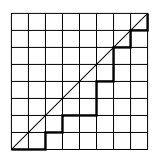
\includegraphics[width=0.5\linewidth]{Photos/Catlan on lattice.png}
        \caption{One such path.}
        
    \end{figure}
    Now let's find the total number of such paths. The total number of lattice paths from $(0, 0)$ to $(n, n)$ without the $x \geq y$ restriction is equal is $\binom{2n}{n}$ using basic PnC. \par
    Using the principle of complementary counting, Let us count the number of paths that go into the $x < y$ region.  They shall be called the bad paths. We'll subtract them later.\par
    Suppose that $P$ is a bad path. Since $P$ goes into the region $x < y$, it must hit the line $y = x + 1$ at some point. Let $X$ be the first point on the path P that lies on the line $y = x + 1$\par
    Now, reflect the portion of path P up to X about the line $y = x + 1$, Keeping the latter portion of P the same. This gives us a new path $P'$. It is trivial to observe that every bad path will have one and only one reflection.\par
    \begin{figure}
        \centering
        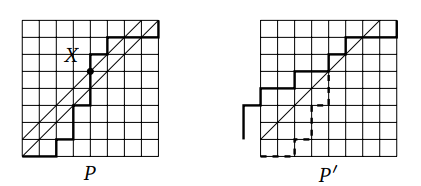
\includegraphics[width=0.5\linewidth]{Photos/Bad path reflection(catlan).png}
        \caption{An example}
        
    \end{figure}
The number of bad paths is therefore equal to the number of lattice paths from $(-1, 1)$ to $(n, n)$ using only unit up and right steps.  Notice, that there is no restriction anymore, so we can compute the number of such paths simply as: $\binom{2n}{n+1}$.\par
So the number of Dyck paths from $(0,0)$ to $(n,n)$ are:\par
$\binom{2n}{n} - \binom{2n}{n+1} = \binom{2n}{n} - \frac{n}{n+1} \binom{2n}{n} = \frac{1}{n+1} \binom{2n}{n}$
\end{proof}
The sequence of such numbers is called the Catalan numbers after the French-Belgian mathematician Eugène Charles Catalan. They come up a lot. The sequence goes like:$1, 2, 5, 14, 42 \dots$. The $n^{th}$ term is(as we derived above):
\begin{theorem}
    $C_n=\frac{1}{n+1} \binom{2n}{n}$
\end{theorem}
\section{Incidence Matrices}
We used the concept of counting in two ways while deriving the identities. In this chapter, we will now learn about incidence matrices and use them to set up the double counting. While the incidence matrix is a very powerful tool, and can solve a lot of questions, we'll see even stronger methods later.\par
\begin{example}
In a certain committee, each member belongs to exactly three subcommittees, and each subcommittee has exactly three members. Prove that the number of members equals to the number of subcommittees.
\end{example}
Here’s how we usually set up the incidence matrix. In our incidence matrix, each row represents a member, and each column represents a subcommittee. An entry is 1 if the member corresponding to its row belongs to the subcommittee corresponding to its column; otherwise, the entry is 0. Of course, the roles of rows and columns may be interchanged without any loss of generality. If we had 5 members,  and 5 subcommittee's, we'd have a matrix looking something like:\par
$\begin{pmatrix}
1 & 1 & 1 & 0 & 0 \\
0 & 0 & 1 & 1 & 1 \\
1 & 0 & 1 & 0 & 1 \\
0 & 1 & 0 & 1 & 1 \\
1 & 1 & 0 & 1 & 0 \\
\end{pmatrix}$\par
Suppose that there are n subcommittees and m members. Then the incidence matrix is a $m \times n$ matrix. The given conditions tell us that each row contains 3 ones, so there are $3m$ ones in total.\par
On the other hand, each column contains 3 ones, so there are $3n$ ones in total. Equating the two counts, we see that $3m = 3n$, so $m = n$, which is what we wanted to prove.\par
The methodology of incidence matrix is based on a simple idea, \textbf{the sum of elements taken one row at a time is equal to sum of elements taken one column at a time.}\par
However, this approach is often not enough. Oftentimes, we are given some restriction that applies to every pair of organizations (or individuals). For example, it may be that every two organizations share exactly one common member. In this case, counting the number of $1$’s as we did above does not incorporate all the given information, and thus would likely be unsuccessful. Fortunately, such problems can usually be approached by counting pairs of $1$’s. Specifically, we are interested in the number of pairs of $1$’s that lie on the same column (or row).\par
\begin{example}
    (IMC 2002) Two hundred students participated in a mathematical contest. They had six problems to solve. It is known that each problem was correctly solved by at least $120$ participants. Prove that there must be two participants such that every problem was solved by at least one of these two students.
\end{example}
\begin{proof}
    Let's assume, to the contrary, that no two students managed to together solve all the problems. That means, for any set of two students, one problem must be unsolved by both.\par
    This prompts us to count the pairs of students with their unsolved problem. Let us consider the incidence matrix of this configuration. We have six rows, each representing a problem, and 200 columns, each representing a student. In light of the above remark, we make an entry of the matrix 1 if the student corresponding to the column did not solve the problem corresponding to the row, and make the entry 0 otherwise. The setup is illustrated below:
    \[ \begin{pmatrix}
1 & 1 & 0 & \dots & 0 & 0 \\
0 & 1 & 1 & \dots & 0 & 0 \\
0 & 0 & 0 & \dots & 1 & 1 \\
0 & 0 & 0 & \dots & 0 & 0 \\
0 & 0 & 0 & \dots & 0 & 1 \\
1 & 0 & 0 & \dots & 0 & 0 \\
\end{pmatrix}\]
Let $T$ denote the set of pairs of $1$ in the same row. We'll be considering the cardinality(fancy way to say number of elements) of the set $T$.\par
Counting by column: As there exists a problem unsolved by any two students, we should have at least a pair of ones in one of the rows if we choose any two columns. Basically, $|T| \geq \binom{200}{2}$.\par
Counting by row: As every problem was solved by at least 120 students, there are at most 80 ones in every row.  So we have $\binom{80}{2}$ pairs of one per row. That means, $|T| \leq 6 \binom{80}{2}$\par
We are done as the above implies: $\binom{200}{2} \leq |T| \leq 6 \binom{80}{2}$, which is false as $\binom{200}{2}  \geq 6 \binom{80}{2}$. Hence, our initial assumption was false. Thus, the converse is true. \par
Hence, proved.\par
\end{proof}
\begin{xcb}{Exercises}
\begin{enumerate}
\item How many ways are there to tile an 10 by 2 board with 1 by 2 dominoes such that each domino covers exactly two squares and no domino overlaps?
\item (BMO 2013) Isaac is planning a nine-day holiday. Every day he will go surfing, or water skiing, or he will rest. On any given day he does just one of these three things. He never does different water-sports on consecutive days. How many schedules are possible for the holiday?
\item  (AIME 2015) There are $2^{10} = 1024$ possible 10-letter strings in which each letter is either an $A$ or a $B$. Find the number of such strings that do not have more than 3 adjacent letters that are identical.
\item Given a regular 2n-gon, how many ways are there to pair vertices and draw line segments between those vertices such that no two line segments intersect?
\item(IMO/6 1979) Let $A$ and $E$ be opposite vertices of an octagon. A frog starts at vertex $A.$ From any vertex except $E$ it jumps to one of the two adjacent vertices. When it reaches $E$ it stops. Let $a_n$ be the number of distinct paths of exactly $n$ jumps ending at $E$. Prove that:\[a_{2n-1}=0, \quad a_{2n}={(2+\sqrt2)^{n-1} - (2-\sqrt2)^{n-1} \over\sqrt2}.\]
\item (AIME 2006) A collection of 8 cubes consists of one cube with edge-length $k$ for each integer $k, 1 \le k \le 8.$ A tower is to be built using all 8 cubes according to the rules:\par
- Any cube may be the bottom cube in the tower.
- The cube immediately on top of a cube with edge-length $k$ must have edge-length at most $k+2.$\par
Let $T$ be the number of different towers than can be constructed. What is the remainder when $T$ is divided by 1000?
\item (ISI 2023) Three left brackets and three right brackets have to be arranged in such a way that if the brackets are serially counted from the left, then the number of right brackets counted is always less than or equal to the number of left brackets counted. In how many ways can this be done? $\clubsuit$ What about for $n$ left brackets and $n$ right brackets.  
\item  Find the number of triangulation's of a convex $(n + 2)$gon into $n$ triangles by $n-1$ diagonals that do not intersect their interiors.
\item (USAMO 1996) An $n$-term sequence $(x_1, x_2, \ldots, x_n)$ in which each term is either 0 or 1 is called a binary sequence of length $n$. Let $a_n$ be the number of binary sequences of length n containing no three consecutive terms equal to 0, 1, 0 in that order. Let $b_n$ be the number of binary sequences of length $n$ that contain no four consecutive terms equal to 0, 0, 1, 1 or 1, 1, 0, 0 in that order. Prove that $b_{n+1} = 2a_n$ for all positive integers $n$.
\item (IOQM 2023) Given a $2 \times 2$ tile and seven dominoes ( $2 \times 1$ tile), find the number of ways of tiling (that is, cover without leaving gaps and without overlapping of any two tiles) a $2 \times 7$ rectangle using some of these tiles.
\item (China 1993) A group of 10 people went to a bookstore. It is known that:\par
1. Everyone bought exactly 3 books\par
2. For every two persons, there is at least one book that both of them bought.\par
What is the least number of people that could have bought the book purchased by the greatest number of people?\par
\item (China 1992) Sixteen students took part in a math competition where every problem was a multiple choice question with four choices. After the contest, it is found that any two students had at most one answer in common. Determine the maximum number of questions
\item  (China 1995) Twenty-one people took a test with 15 true and false questions. It is known that for every two people, there is at least one question that both have answered correctly. Determine the minimum possible number of people that could have correctly answered the question that most number of people are correct on.
\item (China 1996) Eight singers participate in an art festival where $m$ songs are performed. Each song is performed by $4$ singers, and each pair of singers performs together in the same number of songs. Find the smallest $m$ for which this is possible.
\item (AIME 2018) The wheel shown below consists of two circles and five spokes, with a label at each point where a spoke meets a circle. A bug walks along the wheel, starting at point $A$. At every step of the process, the bug walks from one labeled point to an adjacent labeled point. Along the inner circle the bug only walks in a counterclockwise direction, and along the outer circle the bug only walks in a clockwise direction. For example, the bug could travel along the path $AJABCHCHIJA$, which has $10$ steps. Let $n$ be the number of paths with $15$ steps that begin and end at point $A$. Find the remainder when $n$ is divided by $1000.$
\begin{figure}[h]
    \centering
    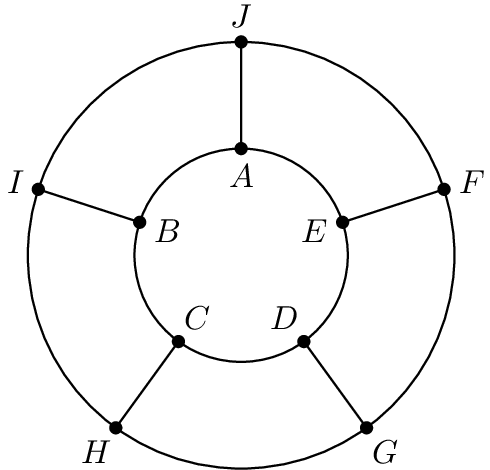
\includegraphics[width=0.5\linewidth]{Photos/AIME 2018.png}
\end{figure}
\item How many $n$-digit numbers whose digits are in the set $\{2, 3, 7, 9\}$ are divisible by $3$?
\end{enumerate}
\end{xcb}